\chapter{Disease detection}

Let me introduce to the topic of my PhD work at \acrfull{sk}.

\todo[inline]{TODO: complete chapter}

\section{Thesis Structure}
The diagram in \autoref{fig:thesis-structure} illustrates the flow of information through the structure of the thesis.

\begin{figure}[htb!]
\centering 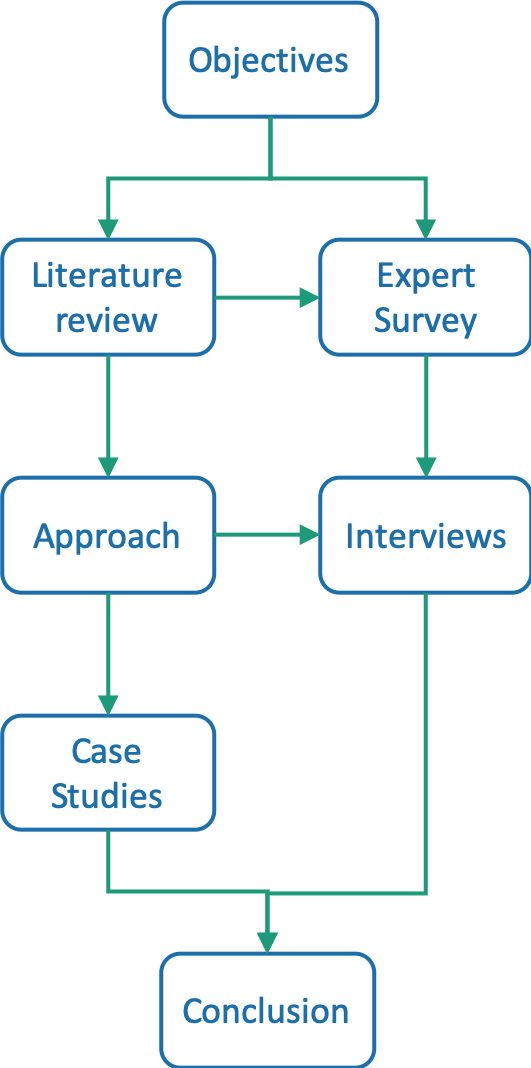
\includegraphics[width=0.5\textwidth]{graphics/thesis-structure}
\caption{Thesis structure}
\label{fig:thesis-structure}
\end{figure}

\begin{description}
    \item[\Autoref{cap:background} - Background]
Here's the literature review.

    \item[\Autoref{cap:thesis_objectives} - Thesis Objectives]
We define the objectives of our work.

...

    \item[\Autoref{cap:conclusion} - Conclusion]
In the last chapter, we discuss our results obtained ...

%%%%%%%%%%%%%%%%%%%%%%%%%%%%%%%%%%%%%%%%%%%%%%

%%%%%%%%%%%%%%%%%%%%%%%%%%%%%%%%%%%%%%%%%%%%%%

%%%%%%%%%%%%%%%%%%%%%%%%%%%%%%%%%%%%%%%%%%%%%%

% =======================================================
%# Modern greenhouses #
% =======================================================
Modern agriculture poses several challenges in terms of the requirements for monitoring speed and precision.
%old sentence
%After a certain size of the greenhouse, that is already reached by several major agricultural companies, it becomes virtually impossible to timely examine the whole greenhouse facility with a reasonable human workforce.
Certain greenhouses of the major agricultural companies are so huge, that it is virtually impossible to timely examine the whole facility with a reasonable human workforce.
While it is possible to introduce more and more human workers, a sustainable long-term solution is to use autonomous robots to automate such repetitive tasks.

While robot-assisted agriculture has been developing for a long time already, the integration of a robot into an industrial-scale production often demands substantial effort.
It requires the robot to have a high degree of autonomy while keeping the modifications that the greenhouse facility should go through to the minimum.
% =======================================================
\subsection{Target environment}
% =======================================================
The target greenhouses for this project are rectangular 120000 \si{m^2} (12 hectares) buildings with glass rooftops.
During the night and in cloudy weather red-blue LEDs are used to provide sufficient lighting.
The temperature and humidity are kept stable at all times. Several types of tomatoes are grown there with the help of hydroponics. One tomato plant grows up to 35 meters in length during 10 months of cultivation.
The majority of the length of the plant is kept horizontal, and the top of the plant is at a height of approximately 4 meters.
% =======================================================
\subsection{Powdery mildew}
% =======================================================
%old sentence
%The density of the biomass (see Figure \ref{fig_greenhouse_top_view}) in these greenhouses allows for cost savings because of the scale of the production, but, on the other hand, it leads to the rapid spread of various kinds of bacterial infections, fungi, viruses, and insects.
The density of the biomass (see Figure \ref{fig_greenhouse_top_view}) in these greenhouses allows for cost savings because of the scale of the production. 
On the other hand, it leads to the rapid spread of various kinds of bacterial infections, fungi, viruses, and insects. Thus, timely monitoring in such greenhouses is crucial.
Powdery mildew is known to infect the lower leaves first and then spread up the plant.
It develops best at temperatures slightly below 30\si{\celsius} and high humidity, which are precisely the conditions that the tomatoes are grown in for the great portion of the production cycle.
Thus, the development of the powdery mildew is rapid, taking 4 to 7 days to progress from early to medium stage \cite{WSPANIALY2016487}.

% =======================================================
%# Robot  #
% =======================================================
\begin{figure}[!htb]
    \centering
    %\begin{subfigure}{0.48\textwidth}
    %    \centering
        \includegraphics[width=0.48\textwidth]{gfx/images/greenhouse/greenhouse_top_view_fixed-2.png}
        \caption{Image taken in a greenhouse at the top of the plants.}
        \label{fig_greenhouse_top_view}
    %\end{subfigure}
\end{figure}
With the aforementioned requirements for monitoring speed in mind, an autonomous robot on an omnidirectional platform was developed and manufactured.
It is equipped with cameras, covering the whole height of the tomato plant, and an onboard computer to process the data in real-time.

This paper presents a work on the data acquisition with this robot, as well as coordinating the markup procedure by human experts and a comparison of the performance of several neural networks.
% =======================================================
%# State of the field
% =======================================================
\subsection{Datasets available and related work}

The majority of the open datasets are either small or taken in laboratory conditions, meaning professional cameras, artificial lighting, separation of the leaves from the plant, or manual preprocessing.
By far the most popular dataset in the field \cite{hughes2015open} consists of images of leaves on a contrastive background.
Collecting such a dataset is expensive, and its usage is limited by the differences between the laboratory and real conditions.

While there are several publicly available datasets out there, relying on them could be risky due to the covariance shift \cite{sugiyama2008direct}.
%old sentence
%The main difficulties for obtaining qualitative and consistent markup are symptom variations, the potential presence of different disorders with similar symptoms, and ill-defined edges, that lead to ambiguity in the markup \cite{barbedo2016review}.
The main difficulties for obtaining qualitative and consistent markup are\cite{barbedo2016review}:
\begin{itemize}
    \item Symptom variations.
    \item The potential presence of different disorders with similar symptoms.
    \item Ill-defined edge cases, leading to the markup ambiguity.
\end{itemize}Taking into account all the aforementioned factors, a dataset for classification, consisting of images from the target greenhouse in normal conditions was collected and marked, see section \ref{Markup}.
It is worth noting that accuracy is by far the most used evaluation metric in the field of automatic plant disease detection \cite{teeffelen2023detection}.

% =======================================================
%# Contribution  #
% =======================================================

\subsection{Related work}

There are multiple solutions to the same problem that were stated in different environments.
They can rely on hyperspectral imaging \cite{zhang2023detection}, \cite{fernandez2021cucumber}, \cite{PowderyZiheng}, \cite{abdulridha2020detecting}, on recurrent NNs \cite{varshney2021deep}, a custom convolutional architecture \cite{lin2019deep}.
Hyperspectral cameras are usually expensive, which limits their availability.
In this work, relatively cheap user-grade RGB cameras were used.

There are several works that are aimed at comparing the performance of already widely adopted models on specific tasks, such as \cite{PowderyBOYAR}, \cite{9566132}, and \cite{augmentationShin}.
The aim of this work is to produce a solution that fits the specific needs of the environment from an engineering standpoint, see section \ref{Overview of the solution}.

\subsection{Contribution}

The contributions of this paper are as follows:
\begin{itemize}
    \item Roboticised data acquisition was performed. Namely, a robot was designed and manufactured, and a dataset of powdery mildew-infected tomato leaves was gathered. The data collection was performed in a real environment under varying lighting conditions.
    \item Marking of the 6817 images into positive and negative classes was coordinated. The markup was performed by human experts with formal education in agriculture. The consistency of the experts was assessed by providing the same samples to different experts.
    \item Using this data, an experiment was conducted: YOLOv8 (n, s, m), EfficientNet (V2l, B3, B4), ResNet (34 and 152), MobileNetV3 (small and large) were compared in terms of their accuracy and the inference time on the target computer.
    \item It was thus demonstrated that good enough performance could be achieved with the means of user-grade cameras and images that were taken from the moving robot. The mutual expert consistencies were matched by the NN model in terms of the classification accuracy, see section \ref{sec_results}.
\end{itemize}

The paper is structured as follows.
First, the mechanical platform is briefly described and an overview of the solution to the disease detection problem is given.
Second, the data acquisition and markup procedures are described.
Third, the training in terms of the models, parameters, and experiments is described.
Finally, a comparison of the performance of different NN models is given.
% =============================================
%# II. Platform #
% =============================================
\section{Platform}
\label{sec:platform}
With a prospective weight of the robot of around 100 kilograms, an aluminum frame made of a profile with a square cross-section was designed.
%old sentence
%The designing of the chassis was performed with the intent to minimize the number of individually actuated elements and ended up with an omnidirectional platform with 4 identical wheel pairs.
The design of the chassis was performed with the intent to minimize the number of individually actuated elements. 
The result is an omnidirectional platform with 4 identical wheel pairs.
%, where the outer one is the Mecanum wheel, and the inner one is a rail wheel with a T-shaped cross-section.

\begin{figure*}[ht!] 
    \centering
    \begin{subfigure}[b]{0.43\textwidth}
        \centering
        \includegraphics[width=\textwidth]{gfx/images/robot/cam_pos_scheme_2.png}
        \caption{}
        \label{fig_camera_positioning}
    \end{subfigure}
    %\hfill
    \begin{subfigure}[b]{0.43\textwidth}
        \centering
        \includegraphics[width=\textwidth]{gfx/images/robot/another_2.png}
        \caption{}
        \label{fig_robot_in_real_world}
    \end{subfigure}
    \caption{(a) Sketched Fields of View of the cameras. (b) Physical assembly during the data acquisition.}
    \label{fig:Robot}
\end{figure*}

%Regarding the power supply of the robot, 6 of 24 \si{A h} 48 \si{V} LiNCA batteries were chosen, resulting in 144 \si{A h} (approximately 7 \si{kW h}) or nearly 14 hours of uptime on one charge with the prospective power consumption of 500 \si{W}.

\blue{
The power supply and consumption of the robot could be summarized as follows:
\begin{itemize}
    \item 6 $\times$ 24 \si{A h} 48 \si{V} LiNCA batteries
    \item 144 \si{A h} (approximately 7 \si{kW h})
    \item Nearly 14 hours of uptime on one charge with the power consumption of 500 \si{W}
\end{itemize}
}

One of the crucial decisions that had to be made was the positioning of the host computer for the NNs inference.
The final design of the robot included a relatively powerful computer on board, see section \ref{sec_training}.
%old sentence
%It could seem reasonable to do that the other way, but separating the whole system into two parts, namely the robot and the external server, will require the installation of the latter, as well as providing coverage of the whole greenhouse with a wireless network, capable of streaming multiple at FullHD videos in real-time.
It would be reasonable to do this in another way – by dividing the system into a robot and an external server.
This would bring the problem of providing coverage of the entire greenhouse with a wireless network capable of broadcasting a number of (at least) FullHD videos in real-time.
% =============================================
%# III. Vision #
% =============================================
%\section*{Vision}
%\subsection*{Overview}
\section{Overview of the solution}
\label{Overview of the solution}
For the problem of tomato greenhouse monitoring the main requirements for the vision system are the following.

First, the combination of the Fields of View (FoV) of the cameras should cover the entire height of the plants, from the tomatoes to the tips of the vegetation.
Diseases, parasites, and damage can occur anywhere on the plant.
This requirement is addressed by installing a number of cameras, their proper positioning, and their parameters.
Three web cameras were utilized.
The sketch of this setup is given in Figure \ref{fig_camera_positioning}, and the real assembly is given in Figure \ref{fig_robot_in_real_world}.
At this point, only one side is covered by combined FoVs, but it is planned to replicate that and cover the other side as well.

%old sentence
%Second, the image processing should be performed in real-time. Ideally, the robot is expected to spend all the time in the field moving, and with real-time processing, it is possible for the workers to rapidly examine specific rows of tomato plants.
Second, the image processing should be performed in real-time. 
Ideally, the robot is expected to spend all the time in the field moving. 
With real-time processing, it is possible for the workers to rapidly examine specific rows of tomato plants.
The robot should be capable of observing the same part of the plant from different locations, meaning that the data processing should happen in real-time with a certain overlap in the frames.

During the design of the vision subsystem, the following assumptions were adopted.
In the initial testing, the robot was moving at a speed of 0.26 \si{m/s}, which is a safe value for indoor applications.
Considering potential acceleration for the sake of faster monitoring, an upper-speed limit could be set to 0.5 \si{m/s}.
The horizontal FoV for the chosen optics covers 1.07 \si{m}.
Thus, moving an object through it from left to right takes nearly 2 \si{s}.
To assure the 5-fold overlap, each of the cameras has to capture an image at least once every 0.4 \si{s}.
That results in the requirement for the processing speed of 8 frames of 1056 $\times$ 1056 pixels per second.
This requirement is met with a huge margin.

\begin{figure}
    \centering

    \begin{subfigure}[b]{0.42\textwidth}
        \centering
        \includegraphics[width=\textwidth]{gfx/images/greenhouse/photo_with_disease_1_2.png}
        \caption{Image of powdery mildew-infected leaves.}
        \label{fig_photo_with_powdery_mildew}
    \end{subfigure}
    \hfill
    \begin{subfigure}[b]{0.42\textwidth}
        \centering
        \includegraphics[width=\textwidth]{gfx/images/greenhouse/photo_with_disease_2_2.png}
        \caption{A scattering of white patches is a clear visual sign of the presence of the disease.}
        \label{fig_photo_with_powdery_mildew_zoomed}
    \end{subfigure}
    \caption{(a) Image from the bottom camera of the robot. (b) Zoomed in.}
    \label{fig_leaves}
\end{figure}
%\ref{fig:camera_positioning}

\section{Data markup and quality evaluation}
\label{Markup}
A set of approximately 300000 images was collected with some of them exhibiting manifestations of the powdery mildew, see Figures \ref{fig_photo_with_powdery_mildew}, \ref{fig_photo_with_powdery_mildew_zoomed}.
%This figure encompasses all feasible frames extracted from individual video segments acquired through passages alongside tomato rows, utilizing three cameras.
In order to obtain a dataset of a reasonable size, every 30-th frame was chosen, resulting in approximately 10000 frames that are uniformly distributed across the entire original dataset.

%This approach was employed to introduce greater diversity in the frames, accounting for the robot's movement speed and the frames captured per second.
%Additionally, this downsampling was implemented to enhance operational efficiency by working with a subset of the dataset, rather than the entire population, thus facilitating more manageable analysis and processing.
The process of the data labeling was organized as follows.
At each of the 4 iterations, each of the experts was provided with 550 images of the tomato leaves, which had to be separated into two classes: negative and positive.
Among these 550 images, there were 500 unique for each expert and 50 images shared by all the experts in order to assess their consistency.
The mutual consistencies of the experts in the subsets are given in Table \ref{Tab:consistencies}.

\begin{table}[ht]
    %\begin{subtable}[h]{0.90\textwidth}
    \centering
    \begin{tabularx}{0.48\textwidth}{ 
        | >{\centering\arraybackslash}X 
        | >{\centering\arraybackslash}X 
        | >{\centering\arraybackslash}X 
        | >{\centering\arraybackslash}X 
        | >{\centering\arraybackslash}X | }
        \hline
    Markers & A & B & C & D  \\ \hline
    A & 1.0 & 0.72 & 0.88 & 0.82 \\ \hline
    B &     & 1.00 & \textbf{0.60} & 0.90 \\ \hline
    C &     &      & 1.00 & \textbf{0.70} \\\hline
    D &     &      &      & 1.00 \\
    \hline
    \end{tabularx}
    \caption*{1 iteration}
    
    %\label{tab:1iter}
    %\end{subtable}

    %\hfill
    %\begin{subtable}[h]{0.90\textwidth}
    \centering
    \centering
    \begin{tabularx}{0.48\textwidth}{ 
        | >{\centering\arraybackslash}X 
        | >{\centering\arraybackslash}X 
        | >{\centering\arraybackslash}X 
        | >{\centering\arraybackslash}X 
        | >{\centering\arraybackslash}X | }
        \hline
    Markers & A & B & C & D  \\ \hline
    A & 1.0 & 0.88 & \textbf{0.68} & 0.96 \\ \hline
    B &      & 1.00 & 0.80 & 0.92 \\ \hline
    C &      &      & 1.00 & 0.72 \\\hline
    D &      &      &      & 1.00 \\
    \hline
    \end{tabularx}
    \caption*{2 iteration}
    %\label{tab:2iter}
    %\end{subtable}

    %\hfill
    %\begin{subtable}[h]{0.90\textwidth}
    \centering
    \centering
    \begin{tabularx}{0.48\textwidth}{ 
        | >{\centering\arraybackslash}X 
        | >{\centering\arraybackslash}X 
        | >{\centering\arraybackslash}X 
        | >{\centering\arraybackslash}X 
        | >{\centering\arraybackslash}X | }
        \hline
    Markers & A & B & C & D  \\ \hline
    A & 1.0 & 0.92 & 0.86 & 0.90 \\ \hline
    B &      & 1.00 & 0.94 & 0.98 \\ \hline
    C &      &      & 1.00 & 0.96 \\\hline
    D &      &      &      & 1.00 \\
    \hline
    \end{tabularx}
    \caption*{3 iteration}
    %\begin{subtable}[h]{0.90\textwidth}
    \centering
    \centering
    \begin{tabularx}{0.48\textwidth}{ 
        | >{\centering\arraybackslash}X 
        | >{\centering\arraybackslash}X 
        | >{\centering\arraybackslash}X 
        | >{\centering\arraybackslash}X 
        | >{\centering\arraybackslash}X | }

        \hline
    Markers & A & B & C & D  \\ \hline
    A & 1.0 & 0.94 & 0.92 & 0.92 \\ \hline
    B &      & 1.00 & 0.89 & 0.86 \\ \hline
    C &      &      & 1.00 & 0.92 \\\hline
    D &      &      &      & 1.00 \\
    \hline
    
    \end{tabularx}
    \caption*{4 iteration}
    %\caption{\label{Tab:consistencies} Each subtable represents one of 4 iterations of the data markup. A, B, C, and D in the tables represent the individual human experts. The number in $ij$-th element of the table represents the share of the matching labels (positive or negative) for the corresponding experts on a subset of 50 images that they shared during that iteration.}
    \caption{\label{Tab:consistencies} \blue{Tables of mutual consistencies of the human experts.} Each table represents one of 4 iterations of the data markup. The consistencies of $0.7$ and below are highlighted in bold. A, B, C, and D in the tables represent individual human experts. The number in $ij$-th element of the table is the fraction of the matching labels (positive or negative) for the corresponding experts on a subset of 50 images that they shared during that iteration. \blue{The mean consistency (excluding the consistency of the experts with themselves) is $0.8579$, which closely matches the accuracy of the best model.}}

\end{table}

It is worth noting, that the major part of inconsistencies occur as a consequence of the frame quality. It is possible to overcome this issue by reducing motion blur with the help of the cameras with a global shutter, however, this work shows that the target problem can be solved with cameras with a rolling shutter.
\section{Training}
\label{sec_training}
\subsection{Hardware}
A two-tier computing strategy for training and testing the neural networks was used.
The training was performed on a stationary server: Intel Core i9-9900 3.10 \si{GHz}, GeForce RTX 3080, 32 \si{Gb}.
Testing was carried out on the target device - the robot's onboard computer. Its performance is much more limited: Intel Core i5-11400H 2.70 \si{GHz}, GeForce RTX 3050Ti laptop, 16 Gb.
Both machines operated under Ubuntu 20.04.

\subsection{Models}
A comparison of 10 top-performing classification models provided by Roboflow \cite{lin2022roboflow} was carried out. These models encompass:

\begin{enumerate}
    \item Three versions of YOLOv8\cite{jocher2022ultralytics}: YOLOv8n, YOLOv8s, and YOLOv8m.
    \item Three versions of EfficientNet\cite{tan2019efficientnet}: EfficientNetV2l, EfficientNetB3 and EfficientNetB4.
    \item Two versions of ResNet\cite{he2016deep}: ResNet34 and ResNet152.
    \item Two versions of MobileNet\cite{howard2017mobilenets}: MobileNetV3small and MobileNetV3large.
\end{enumerate}

\subsection{Data sampling}
\label{Data_sampling}
Three distinct datasets were created, each addressing the class imbalance challenge within the original dataset. Initially, the data comprised 5684 instances of the negative class and 1133 instances of the positive class.
To tackle the imbalance, three different strategies were pursued:
\begin{itemize}
    \item For the first set 1133 images of the negative class were randomly selected, equalizing the number of photos in both classes.
    \item For the second set all the photos from the positive class were duplicated to increase the number of original images of the negative class. The number of training photos per class grew from 850 to 1700.
    \item For the third set, all the labeled data available was used. To achieve this, extensive and diverse augmentation techniques were applied. The positive class images were duplicated six times with augmentation, and similar augmentation transforms were applied to $\frac{6}{7}$ of the negative class images. This training set consists of 5361 instances of the positive class and 5316 instances of the negative class.
\end{itemize}

In all the experiments 75-15-10 \% train-val-test split was used.
\subsection{Data Preprocessing}
\textit{Resizing}: All the images underwent cropping to a square shape and a resizing process with the resultant dimensions of 1056 $\times$ 1056 pixels.
The rationale behind adopting this specific size is the following.
First, some of NN models that were planned to be used could work only with the image sizes that are multiples of 32.
Second, the downscaling of the images was not feasible, because powdery mildew appears with quite small features, and reducing the image size would entail a substantial loss of critical information.
Third, resizing rectangular images into a square will again lead to the loss of data.

%This premise finds empirical validation in the presented tabular data.
%TODO table of comp yolo with diff size(?)
\textit{Augmentation}: Across all three datasets, a standardized suite of transformations was applied.
These transformations encompassed horizontal and vertical flipping, shifting, rotation, and HSV color transformation.
However, it is worth noting that the third dataset underwent a more expansive augmentation strategy.
For this subset, the following augmentations were applied:
\begin{itemize}
    \item \textit{Predominantly:} Defocus, stochastic mist, noise injection, RandomBrightnessContrast, and HSV color transformation featuring augmented values.
    \item \textit{To a smaller extent:} ColorJitter, rgbshift, ChannelShuffle, ChannelDropout, image inversion, and sepia.
\end{itemize}
The selection of these augmentation techniques aimed to diversify the dataset as much as possible to enhance the model's generalization capabilities.
\subsection {Experimental setup}

\blue{
The setup in terms of the training is the following:
\begin{itemize}
    \item Training the majority of the models for 40 epochs before choosing the best checkpoint. The exact number for each model is given in the table \ref{tabularx:models}.
    \item SGD optimizer was used.
    \item The default values for the learning rate of 0.01 for YOLO models and 0.001 for other models were used.
\end{itemize}
}

The choice on the number of epochs was made following preliminary training runs with the learning curves stagnating after such a number of epochs.
The batch size for all models was determined out of the memory constraints.

%In the majority of the experiments, the training was conducted for a total of 40 epochs.
%This number of epochs was deemed sufficient to achieve a consistent learning trajectory even in the presence of noise in the data.
%As for the learning rate, the default values of 0.01 for YOLO models and 0.001 for other models were adopted with the stochastic gradient descent (SGD) optimizer.
%The initial learning rate is a critical hyperparameter that can significantly impact the training process.
%These values served as reasonable starting points, but further fine-tuning and optimization of the learning rate may be necessary, depending on the specific characteristics of the dataset and training dynamics.
%Overall, the chosen approach involved an initial selection of hyperparameter values based on empirical insights and common defaults, followed by iterative experimentation and analysis of the training results to ensure optimal model performance.
%This methodology is consistent with the best practices in deep learning model development and training.
% =============================================
%# III. Results #
% =============================================
\section{Results}
\label{sec_results}
\begin{table*}[!htb]
    \centering    
    \begin{tabularx}{1.0\textwidth}{ 
    | >{\centering\arraybackslash}X 
    | >{\centering\arraybackslash}X 
    | >{\centering\arraybackslash}X 
    | >{\centering\arraybackslash}X 
    | >{\centering\arraybackslash}X 
    | >{\centering\arraybackslash}X 
    | >{\centering\arraybackslash}X | }
    \hline
    Model & Params & Accuracy [\%] & Server inference[ms] & Onboard PC inference[ms] \
    & Training time & Epochs \\ \hline
    Resnet34 & 21.8M & 84.40 & 34.7 & 38.23 & 169m 40s & 40 \\ \hline
    Resnet152 & 60.2M & 85.40 & 34.00 & - & 96m 58s & 40 \\ \hline
    YOLOv8n & 3.2M & \textbf{85.80} & 5.9 & \textbf{6.6} & 25m 54s & 30 \\ \hline
    YOLOv8s & 11.2M & 85.00 & 10.6  & 12.5 & 27m 37s & 30 \\ \hline
    YOLOv8m & 25.9M & 84.50 & 30.7 & 33.0 & 29m 40s & 30 \\ \hline
    %EfficientNet & 19.3M & 85.40 & 35.1 & 178m 46 s & 40 \\\hline
    EfficientNetV2l & 118.5M & 84.07 & 49.3 & - & 124m 19s & 40 \\ \hline
    EfficientNetB3 & 12.2M & 80.53 & 14.86 & - & 66m 45s & 40 \\ \hline
    EfficientNetB4 & 19.3M & 79.20 & 19.7 & - & 74m 29s & 40 \\ \hline
    MobilenetV3small & 2.5M & 83.63 & 4.15 & 6.64 &  54m 23s & 40 \\ \hline
    MobilenetV3large & 5.5M & 84.51 & 4.81 & 19.21 & 52m 23s & 40 \\ \hline
    \end{tabularx}
    \caption{The performance of all models on the first dataset.}
    \label{tabularx:models}
    \begin{tabularx}{1.0\textwidth}{ 
        | >{\centering\arraybackslash}X 
        | >{\centering\arraybackslash}X 
        | >{\centering\arraybackslash}X 
        | >{\centering\arraybackslash}X 
        | >{\centering\arraybackslash}X 
        | >{\centering\arraybackslash}X 
        | >{\centering\arraybackslash}X | }
        \hline
    Model & Accuracy & Inference server (ms) & 
    Inference (ms) & Training time & Epochs & Batch \\ \hline
    YOLOv8n & 85.4 & 5.9 & 6.6 & 83m 52s & 40 & 16 \\ \hline
    MobilenetV3small & 84.07 & 4.2 & 6.61 & 182m 59s & 40 & 32 \\\hline
    MobilenetV3large & 82.74 & 4.87 & 19.41 & 357m 19s  & 40 & 32 \\
    \hline
    \end{tabularx}
    \caption{The performance of the selected models on the second dataset.}
    \label{tabularx:models_extended_dataset}
    \begin{tabularx}{0.99\textwidth}{ 
        | >{\centering\arraybackslash}X 
        | >{\centering\arraybackslash}X 
        | >{\centering\arraybackslash}X 
        | >{\centering\arraybackslash}X 
        | >{\centering\arraybackslash}X 
        | >{\centering\arraybackslash}X 
        | >{\centering\arraybackslash}X | }
        \hline
    Model & Accuracy & Inference server (ms) &
    Inference (ms) & Training time & Epochs & Batch  \\ \hline
    YOLOv8n & 77.5 & 3.3 & 7.3 & 472m 32s & 40 & 16 \\ \hline
    MobilenetV3small & 77.45 & 4.08 & 6.65 &  293m 1s & 40 & 16\\\hline
    MobilenetV3large & 77.45 & 4.95 & 19.16 & 321m 32s & 40 & 16\\
    \hline
    \end{tabularx}
    \caption{The performance of the selected models on the third dataset.}
    \label{tabularx:models_aug_dataset}
%\end{table}
%\end{minipage}
%\begin{minipage}{0.0\textwidth}
%\end{minipage}
\end{table*}
%We trained these models on the first version of the dataset with the fewest photos.
%The training took place on the server and the resulting model was run on the on-board computer.
%For those models for which it was possible to launch the inference, the inference time is indicated on the onboard computer.
%The remaining models were loaded into video memory, but it was not possible to make an inference on them.
%Since we are only interested in what we have done with the possible engineering on the onboard computer, that the models we have chosen have made the network and Resnet152 effective, we do not evaluate the distance.
%We also decided not to consider YOLOv8m and Resnet34 due to the fact that they do not give more accuracy than the remaining MobileNet and Yolo sites while having a much longer inference time.
%Thus, we chose 4 models: YOLOv8n and YOLOv8s mobilenet small and mobilenet large. \ref{fig:First result}

\blue{Overall, a dataset of powdery mildew-infected leaves was collected with the user-grade RGB cameras.
A number of neural networks were trained with the best of them performing on par with the human experts.
The inference time on the onboard computer is well below the maximal acceptable time, thus leaving room for the introduction of other models or increasing the number of cameras.}



%Further experiments were carried out with them.
\begin{figure}[ht] 
    \centering
    \includegraphics[width=0.4\textwidth]{gfx/images/vision_models/acc_fps/server_models.pdf}
    \caption{Performance and FPS of the models trained on the first dataset with inference on the server.}
    \label{fig:Firstresult}
\end{figure}
\begin{figure}[ht] 
    \centering
    \includegraphics[width=0.41\textwidth]{gfx/images/vision_models/acc_fps/laptop_models.pdf}
    \caption{Performance and FPS of the chosen best models trained on the first dataset with inference on the onboard laptop.}
    \label{fig:Secondresult}
\end{figure}


Table \ref{tabularx:models} presents the results of the training of all the models considered on the first version of the dataset, see Section \ref{Data_sampling}.
It was not possible to run certain models on the onboard laptop, \blue{taking into account the target resolution of 1056 $\times$ 1056}. These models are marked with a dash sign in the \textit{Onboard PC inference} column.
These models were excluded from further experiments because they were too demanding in terms of computational resources.
%The remaining models were examined from the standpoint of the combination of accuracy and inference time, see Figure \ref{fig:Firstresult} for results on the server and Figure \ref{fig:Secondresult} for results on the target machine.

All the models were examined from the standpoint of the combination of accuracy and inference time, see Figure \ref{fig:Firstresult} for the results on the server.
It turns out, that three of them are Pareto-optimal, meaning that no other model is faster and more precise at the same time.
Those are YOLOv8n, MobilenetV3small and MobilenetV3large.
Figure \ref{fig:Secondresult} gives their results on the target machine.

%The second version of the dataset includes more original photos of the negative class and duplicates of photos of the positive class.
%Due to the increase in the size of the dataset, the training time has also increased.
%At the same time, the accuracy increased only for the Mobile net V3 small model. \ref{fig:Second result}

Another series of experiments was carried out with three aforementioned models and the second version of the dataset, see Table \ref{tabularx:models_extended_dataset}.
The results did not subvert the expectations with accuracy slightly increasing for MobilenetV3small and slightly dropping for other models.

With the third version of the dataset the accuracy values have become significantly worse, see Table \ref{tabularx:models_aug_dataset}.
The values of the metrics for different models are relatively close to each other, \blue{matching} the consistency of the experts in terms of accuracy.
Thus, the reasonable qualitative explanation could be that the performance is limited more or less by the data quality, not the models' generalization capabilities.
The best performance by both accuracy and time was shown by YOLOv8n neural network.
The False Negative rate for it is 6 \%.

In order to assess the model performance on the high-quality data, a set of 100 images was labeled by a consensus of 4 experts.
The consensus here means that the image-wise labels were agreed upon by all the experts.
The output of the model matched the expert labeling for 96 samples of 100.

The overall performance in terms of speed is well above the minimal requirements, meaning that the monitoring speed is limited by the robot's motion (because of safety concerns), not by the inference time of the neural networks.

\blue{It is worth noting that this excessive performance could be beneficial for solving other related problems. For instance, to detect certain tiny insects it will be necessary to install much more cameras with small FoV. Their number could rise to dozens, requiring very low inference time for a single image. These cases could be addressed without any substantial modification to the vision pipeline.}

% ==================
%# IV. CONCLUSION #
% ==================
\section{Conclusion and future work}

\subsection{Conclusion}

An autonomous agricultural robot on an omnidirectional platform was designed, prototyped, and tested in a real environment.
The camera's positioning allows for the examination of the whole tomato plant, and the onboard computer is capable of processing the data in real-time.

A dataset of powdery mildew-infected tomato leaves was collected, labeled and assessed in terms of consistency. It contains a sufficient amount of data for training modern neural networks of reasonable size, which makes it useful for further industrial applications.

Several modern neural networks were trained for classification and compared on two test sets with one of them being marked by a consensus of experts.
The performance of the models is sufficient and matches with the mutual consistencies of the human experts.

\blue{It was demonstrated that real-time disease recognition could be performed on the robot while moving with the means of the user-grade cameras.
The main limitation of the chosen approach is that RGB cameras require sufficient lighting to function properly.
However, in the given circumstances this requirement is naturally met.}

\subsection{Future work}

The next steps in this project are planned to be the following.
First, the robot requires certain polishing and finalization in terms of mechanics.
In order for it to be constantly deployed in a humid environment it should be watertight.
On the other hand, isolating the inner volume from the environment will require heat dissipation to be reconsidered.

Second, the cameras are supposed to be substituted by a global shutter-based one.
It will practically eliminate the motion blur while requiring certain modifications to the data transfer subsystem.
Moreover, the production-ready version of the camera poles has to be manufactured.
It is supposed to hold the cameras with the help of a mechanism that allows for vertical and horizontal position adjustment.

Third, high-level control should be implemented in the system for the robot to be capable of localizing itself and autonomously following the trajectory set by the user.

Fourth, a Graphical User Interface should be implemented for the end user to control the robot without substantial UNIX knowledge.

Finally, more disease types and crop types should be introduced into the vision subsystem.

\end{description}

